% (The MIT License)
%
% Copyright (c) 2023-2024 Yegor Bugayenko
%
% Permission is hereby granted, free of charge, to any person obtaining a copy
% of this software and associated documentation files (the 'Software'), to deal
% in the Software without restriction, including without limitation the rights
% to use, copy, modify, merge, publish, distribute, sublicense, and/or sell
% copies of the Software, and to permit persons to whom the Software is
% furnished to do so, subject to the following conditions:
%
% The above copyright notice and this permission notice shall be included in all
% copies or substantial portions of the Software.
%
% THE SOFTWARE IS PROVIDED 'AS IS', WITHOUT WARRANTY OF ANY KIND, EXPRESS OR
% IMPLIED, INCLUDING BUT NOT LIMITED TO THE WARRANTIES OF MERCHANTABILITY,
% FITNESS FOR A PARTICULAR PURPOSE AND NONINFRINGEMENT. IN NO EVENT SHALL THE
% AUTHORS OR COPYRIGHT HOLDERS BE LIABLE FOR ANY CLAIM, DAMAGES OR OTHER
% LIABILITY, WHETHER IN AN ACTION OF CONTRACT, TORT OR OTHERWISE, ARISING FROM,
% OUT OF OR IN CONNECTION WITH THE SOFTWARE OR THE USE OR OTHER DEALINGS IN THE
% SOFTWARE.

\documentclass{article}
\usepackage{../sqm}
\newcommand*\thetitle{Neural Metrics}
\begin{document}

\plush{\sqmTitlePage{24}{}}

\qte
  [Michael Pradel and Satish Chandra]
  {michael-pradel.jpg}
  {\ul{Neural} software analysis offers a fresh approach, enhancing or even \ul{surpassing} traditional program analysis in some areas.}
  {pradel2022}

\qte
  [Martin White]
  {martin-white.jpg}
  {Among the true positives, we found pairs mapping to all four clone types. We compared our approach to a traditional structure-oriented technique and found that our learning-based approach \ul{detected clones} that were either undetected or suboptimally reported by the prominent tool Deckard.}
  {white2016deep}

\qte
  [Pavol Bielik]
  {pavol-bielik.jpg}
  {In this paper we present a new, automated approach for creating static analyzers: instead of manually providing the various inference rules of the analyzer, the key idea is to \ul{learn} these \ul{rules} from a \ul{dataset} of programs.}
  {bielik2017learning}

\qte
  [Tomas Mikolov]
  {tomas-mikolov.jpg}
  {The meanings of `Canada' and `Air' cannot be easily combined to obtain `Air Canada'. Motivated by this example, we present a simple method for finding phrases in text, and show that learning good \ul{vector representations} for millions of phrases is possible.}
  {mikolov2013distributed}
\qte
  [Koushik Sen]
  {koushik-sen.jpg}
  {This paper presents DeepBugs, a learning approach to name-based bug detection, which reasons about names based on a semantic representation and which automatically learns bug detectors instead of manually writing them. We formulate bug detection as a \ul{binary classification problem} and train a classifier that distinguishes \ul{correct} from \ul{incorrect} code.}
  {pradel2018deepbugs}

\qte
  [Uri Alon]
  {uri-alon.jpg}
  {\textbf{code2vec}: The main idea is to represent a code snippet as a single fixed-length \ul{code vector}, which can be used to \ul{predict} semantic properties of the snippet.}
  {alon2019code2vec}
\pitch{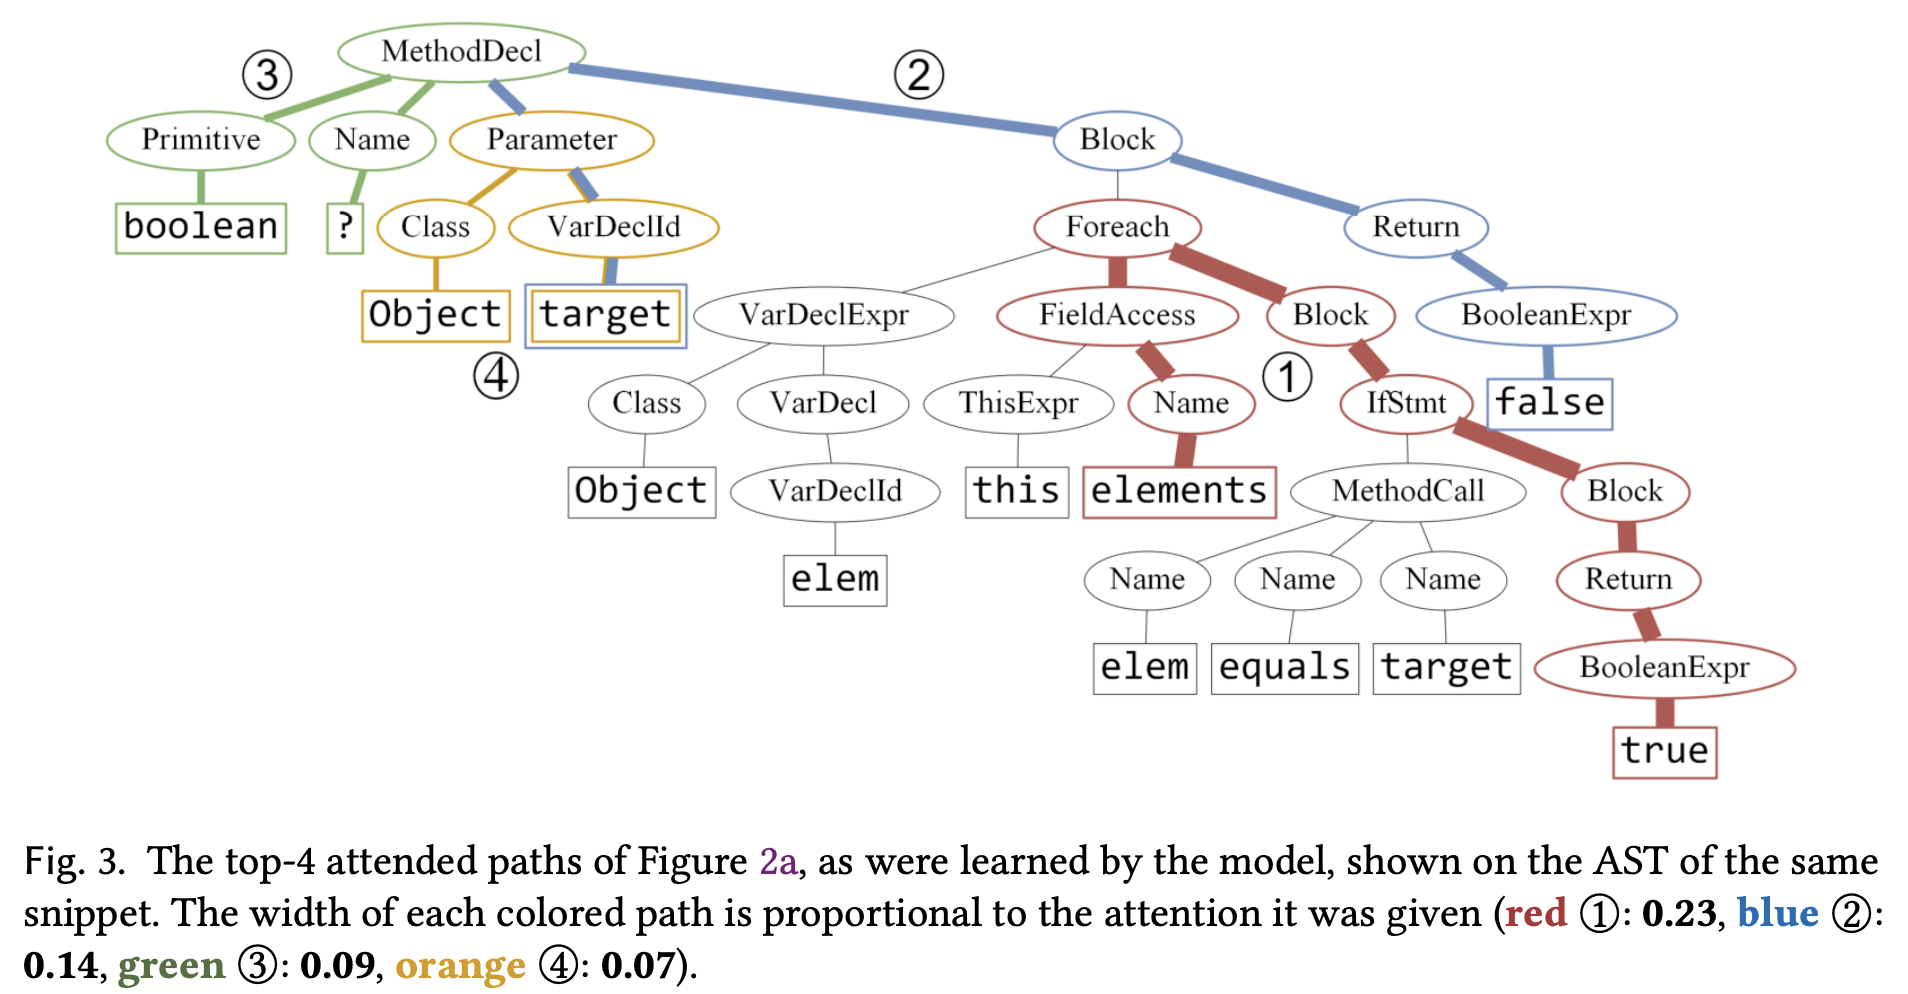
\includegraphics[width=.85\linewidth]{code2vec-1.png}
  \source{alon2019code2vec}}
\pitch{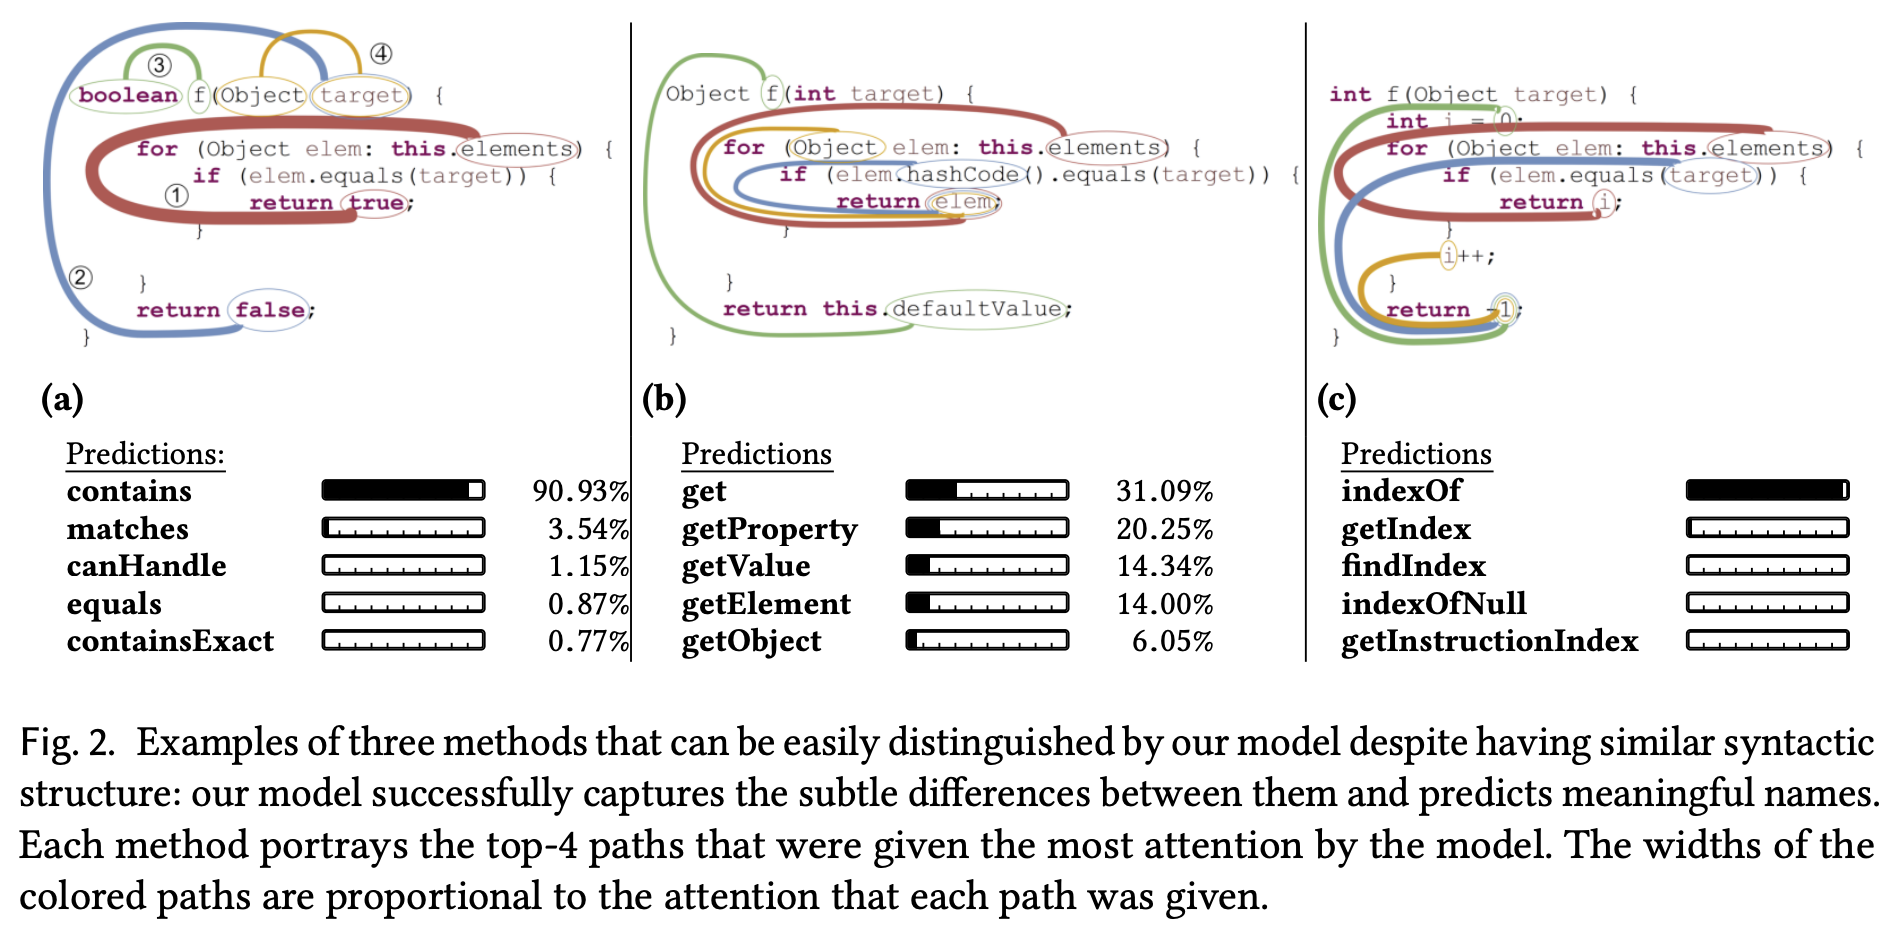
\includegraphics[width=.95\linewidth]{code2vec-2.png}
  \source{alon2019code2vec}}

\qte
  [Mohammad Mahdi Mohajer]
  {mohammad-mahdi-mohajer.jpg}
  {SkipAnalyzer consists of three components, 1) an LLM-based static bug detector that scans source code and reports specific types of bugs, 2) an LLM-based false positive filter, and 3) an LLM-based patch generator that can generate patches for the detected bugs above. As a proof-of-concept, SkipAnalyzer is built on \ul{ChatGPT}.}
  {mohajer2023skipanalyzer}

\qte
  [Haonan Li]
  {haonan-li.jpg}
  {UBITect produces many \ul{false positives} from the static analysis. With a pilot study of 20 false positives, we can successfully \ul{prune} 8 out of 20 based on GPT-3.5, whereas GPT-4 had a near-perfect result of 16 out of 20.}
  {li2023assisting}

\qte
  [Elif Nur Haner K{\i}r{\u{g}}{\i}l]
  {elif-kirgil.jpg}
  {In the study, the \ul{cohesion} value, which is one of the most important criteria for evaluating software quality, was predicted by RF, KNN, REPTree, SVM, MLP, and LR \ul{machine learning} techniques.}
  {haner2023predicting}

\pitch{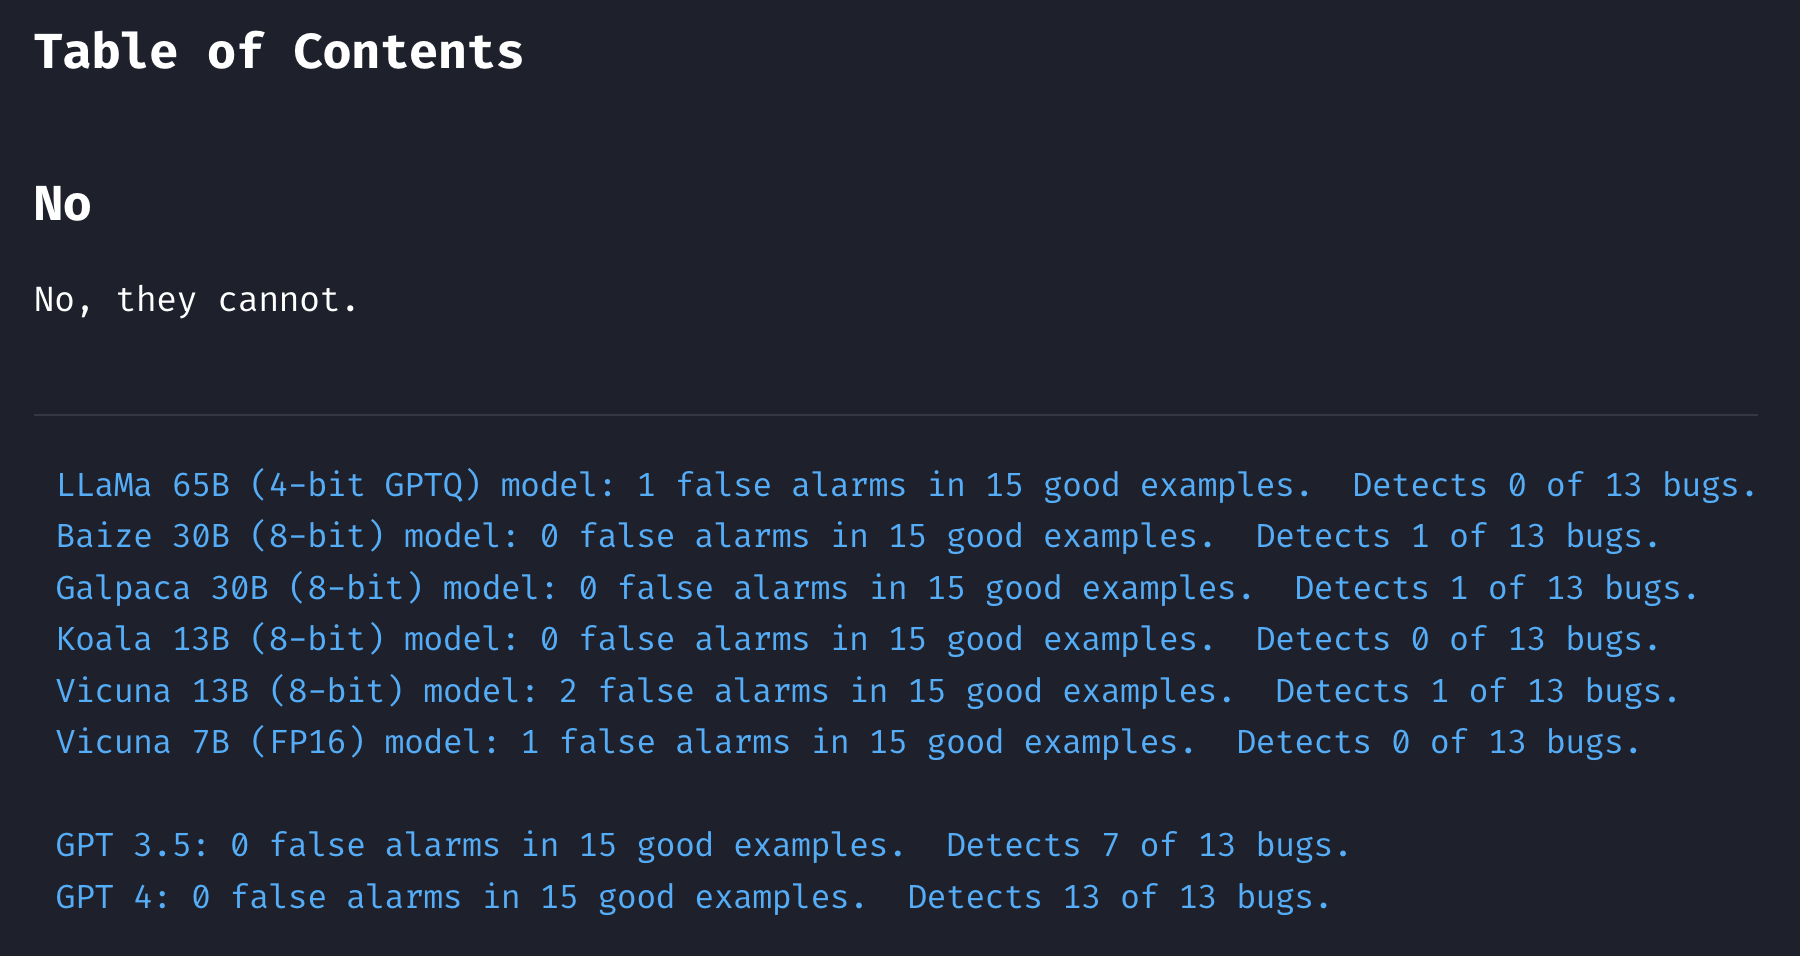
\includegraphics[width=.7\linewidth]{catid.png}
  \source{taylor2023}}

\end{document}
